\documentclass[fr,license=none]{../../../eplnotes}

\usepackage{graphicx}

\usepackage{wasysym}%intégrale double sur contour fermé
\newcommand{\rot}{\vv{\mathrm{rot}}\;}
\newcommand{\divt}{\mathrm{div}\;}
\newcommand{\gradt}{\vv{\mathrm{grad}}\;}

\hypertitle{Math\'ematique}{2}{FSAB}{1102}
{Antoine Leeman}
{François Glineur, Roland Keunings et Enrico Vitale}

\graphicspath{{CM1/}}
\part{Cours Magistral 1 -- Les intégrales multiples}
\section*{Introduction}
\emph{Livre de référence : Calculus Adams}
Les théorèmes ne sont pas démontrés par manque de temps mais ils sont tout de même intéressants.
\section{Intégrales multiples}

Cette section se réfère au chapitre 14 du livre de référence.
\subsection{Introduction}
\[\int_{a}^{b} {f(x) dx}\]


\begin{enumerate}

\item Partition P du domaine $D=[a,b]$
$$ P = \{x_0,x_1,\dots,x_n\}$$
$$a=x_0<x_1<\dots<x_n=b$$
\item On définit la norme de P
$$||P|| = \underset{1\le i \le n}{\max} \overbrace{(x_i-x_{i-1})}^{\Delta x_i}=1$$

\item Dans chaque $[{x_{i-1},x_i}]$ : on choisit un point $c_i$ avec $c=(c_1,c_2,\dots,c_n)$

\item  Somme de Riemann : $$R(f,P,c)=\sum_{i=1}^{n} \overbrace{f(c_i)\dot \Delta  x_i}^{\textbf{aire du rectangle i}} $$

\item Passage à la limite $$\lim\limits_{\substack{||P|| \to 0 \\ n \to \infty}} R(f,P,c) =\int_{a}^{b} {f(x) \dif x}$$

\end{enumerate}
Si cette limite existe, quels que soient les points $c_i$, alors on dira que cette fonction est intégrable.
\begin{myrem}
$$\int_{a}^{b} {f(x) \dif x} = \int_{a}^{b} {f(t) \dif t} = \int_{a}^{b} {f(\alpha) \dif \alpha}$$ où $f(x)$ représente l'intégrand et $\dif x$ représente la variable d'intégration \textit{\og dummy variable \fg{}}.
\end{myrem}

\begin{myrem}

Les courbes sous l'axe sont négatives et au-dessus sont positives. On additionne le tout. On peut donc avoir une somme d'aire négative.

$$\int_{a}^{b} {f(x) \dif x} \quad D=[a,b] \subset \mathbb{R}^1$$
$$\int_D f(x_1,x_2,\dots,x_n) \dif x_1 \dots \dif x_n \quad D \in \mathbb{R}^n$$
La généralisation de $n=1$ à $n=2$ n'est pas évidente, mais la généralisation de $n=2$ à $n=\infty$ est plus simple, étrangement.
\end{myrem}

\subsection{Intégrale Double}
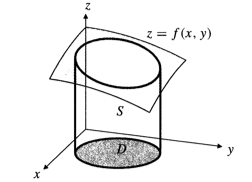
\includegraphics[scale=1]{image3.png}

Région solide $ S \subset \mathbb{R}^3$
\[I=\int \limits_{D} f = \iint_D f (x,y) \dif A\]
$\dif A$ est un élément d'aire infinitésimale. L'écriture avec une seule intégrale et uniquement l'intégrant est la notation \og matheuse\fg{}, l'écriture avec autant d'intégrales que de dimensions, et avec le $\dif A$, est la notation \og ingénieur\fg{}.

$(f \ge 0) \Rightarrow I = \text{Volume de S}$

Développons un peu\dots
\begin{enumerate}
\item

$$D= \text{``pavé'' dans }\mathbb{R}^2 = [a,b]\times[c,d]$$

Chaque rectangle est appelé $R_{ij}$, avec \(1 \le i \le m\) et \(1 \le j \le n\)

$$R_{ij}=[x_{i-1},x_i]\times[y_{j-1},y_j]$$
L'aire de $R_{ij}$ vaut donc
$$R_{ij}=[x_{i-1},x_i] \cdot [y_{j-1},y_j]= \Delta x_i \Delta y_j$$

\item{Norme de P}

diag = diamètre $R_{ij}= \sqrt{\Delta x_i^2+\Delta y_j^2}$


\item


\textit{Dans chaque $R_{ij}$, on choisit un point}
$$\{c_{ij}^* = (x_{ij}^*,y_{ij}^*)\} = C^*$$

\item
$$R(f, P,c^*)=\sum_{i=1}^{m} \sum_{j=1}^{n} f(x_{ij}^*,y_{ij}^*)\Delta A_{ij}$$
Avec $\Delta A_{ij}$ qui vaut $\Delta x_i \Delta y_j$

\item

$$\lim\limits_{\substack{\norm{P} \to 0 \\ n \to \infty\\ m \to \infty}} R(f,P,c^*)=\int_D f$$

\end{enumerate}

\begin{mytheo}

Si f est continue sur $D$, alors f est intégrable sur $D$. C'est vrai aussi pour toutes les dimensions ! C'est une condition suffisante (l'inverse n'est pas vrai).

C'est-à-dire une fonction non-continue peut être intégrable.

\end{mytheo}

\subsection{ Généralisation à $D$ borné }

\subsubsection{ Dans $ \mathbb{R}^2$ }

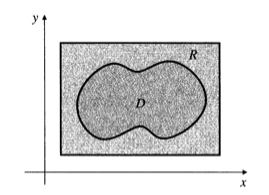
\includegraphics[scale=1]{image4.png}

Rectangle qui contient le domaine D et dont les côtés sont parallèles aux axes.
\[\hat{f} = \text{ extension f de D à } \mathbb{R^2}\]

\[
\hat{f}(x,y)
\begin{cases}
f(x, y) & \text{si } (x, y) \in D \\
0 & \text{sinon} \\
\end{cases}%\left\{
%\begin{array}{l r}
%f(x,y)\text{ si }(x,y)\in D\\
%0\text{ sinon}\\
%\end{array}
%\right.
\]

$f$ intégrable sur D $ \Longleftrightarrow \hat{f}$ intégrable sur $\mathbb{R^2}$ et alors
$\int_D f \eqdef \int_R \hat{f} $


On peut appliquer maintenant pour $n$ :
\\
$ D \subset \mathbb{R}^n$
$$\int_D f = \overbrace{\iint \dots}^\text{$n$-uple} \int_D f(x_1,x_2,\dots,x_n) \dif x_1 \dif x_2 \dots \dif x_n $$

Le produit des $\dif x_1 \dots \dif x_n $ qui sont des éléments infinitésimaux de volume

\subsubsection{Dans $\mathbb{R}^3$}

D = boite de $\mathbb{R}^3$ avec les faces parallèles aux plans de coordonnées\\

Il faut faire un découpage en sous-boîtes $ R_{ijk} $ de taille $\Delta x_i \Delta y_j \Delta z_k$

$\left\{
\begin{array}{l}
1 \le i \le m \\
1 \le j \le n \\
1 \le k \le l \\
\end{array}
\right. $

Il faut choisir \[C_{ijk}^* \in R_{ijk} ( x_{ijk}^*,y_{ijk}^*,z_{ijk}^*)\]

\[R(f,P,c^*)=\sum_{i=1}^m \sum_{j=1}^n\sum_{k=1}^l f (x_{ijk}^*,y_{ijk}^*,z_{ijk}^*) \Delta V_{ijk}\]

On aura donc que

$$\lim\limits_{\substack{l \to \infty \\ n \to \infty\\ m \to \infty}} R=\int_D f$$

Solide borné de $\mathbb{R}^3$
\[\hat{f}=
\begin{cases}
f & \text{si } (x, y, z) \in D \\
0 & \text{sinon} \\
\end{cases}
\]

\[\int_D f \eqdef \int_R \hat{f}\]
\emph{
Donc, lorsque le domaine de définition d'une intégrale est borné dans $\mathbb{R}^2$ ou $\mathbb{R}^3$, on peut étendre ce domaine à condition de poser que les points qui n'appartiennent pas à ce domaine valent $0$.}
\subsection{Propriétés}

\[\int_D f \text{ avec D borné sur } \mathbb{R}^n\]

\begin{myprop}
$f\equiv 1 $
\[\text{D borné de }\mathbb{R}^n\]
\[n=1 : D=[a,b] \int_a^b 1 = b-a = \text{Longueur de }D\]
\[n=2 : D=[a,b]\times[c,d] \int_a^b \int_c^d 1 = (b-a) \cdot (d-c)= \text{Aire de }D\]

\[n=3 : \int_D 1 = \text{Volume de }D\]

Et ainsi de suite. Il suffit d'intégrer la fonction $f(x) = 1$ pour connaître la longueur, la surface, le volume, etc. du domaine.
\end{myprop}


\begin{myprop}
$\forall L,M \in \mathbb{R} ,\forall f,g$ intégrable sur $D \subset \mathbb{R}^n$


\[\int_D(Lf+Mg)\overset{?}{=}L\int_D f + M \int_D g\]
On effectue un déplacement linéaire de l'intégrale. L'intégrale étant une fonction linéaire, cette égalité est justifiée !

\end{myprop}


\begin{myprop}
$$\text{Si } f \le  g  \text{ } \forall \text{ point de }D\subset \mathbb{R}^n \text{alors} \int_D f \le \int_D g $$
Cette propriété se vérifie très facilement de manière géométrique.
\end{myprop}

\begin{myprop}
$D= D_1 \cup D_2 \cup \cdots \cup D_k$ et $D_i \cup D_j = \varnothing$ et $i\neq j$ non-overlapping

On aura donc que l'intégrale sur $D_i$ de $f$ est
\[\int_D f=\sum_{j=1}^k \int_{D_j} f\]

On peut découper le domaine D en plusieurs sous-domaines distincts et calculer la somme des intégrales sur chacun des sous-domaines.
\end{myprop}

\begin{myprop}
\[\abs{\int_D f} \le \int_D\abs{f}\]

La valeur absolue de l'intégrale de f sera toujours plus petite que l'intégrale de la valeur absolue de f. Encore une fois, on voit cela très rapidement de manière géométrique. C'est une généralisation de l'inégalité triangulaire.
\end{myprop}

\begin{myprop}[Théorème de Fubini :]
\emph{Ce théorème ne se trouve pas dans le livre !}
Il permet de \strong{réduire} le calcul d'une intégrale $n$-uple à une \strong{succession} (dans l'ordre qui convient le mieux) de n intégrales \strong{unidimensionelles}.

\textit{\textbf{Enoncé}} \\Soit $f$ définie sur un pavé D de $\mathbb{R}^n$\\
$D=[a_1,b_1]\times[a_2,b_2]\times \cdots\ \times[a_n,b_n]$

\[f(x_1,x_2,\cdots,x_n) : D\to\mathbb{R}\]
Si $f$ est continue sur D, alors : $(\sigma(1),\sigma(2),...,\sigma(n)) $ = une permutation quelconque de (1,2,...,n)

$$
\int_D f= \int_{a_{\sigma(1)}}^{b{\sigma(1)}}
\left[
\int_{a_{\sigma(2)}}^{b{\sigma(2)}}
\left[ \cdots\ \left[
\int_{a_{\sigma(n)}}^{b{\sigma(n)}}
f(x_1,x_2,\cdots,x_n )\dif x_{\sigma(n)}
\right]\cdots\right]
\dif x_{\sigma(2)} \right] \dif x_{\sigma(1)}
$$

Si la fonction f est \textbf{continue}, on peut calculer les intégrales les unes après les autres dans l'ordre de notre choix en considérant les autres variables comme des constantes.
\end{myprop}




\subsubsection{Illustration du Théorème de Fubini pour $n=2$}




$ \left\{
\begin{array}{l}
D = [0,2]\times[1,3]\\
f = x^2+y
\end{array}
\right.
$

$
 \left\{
\begin{array}{l}
x_1=x\\
x_2=y
\end{array}
\right.
$
$(1,2)=(\sigma(1),\sigma(2))$

\[\int_D f = \int_0^2 \left[ \overbrace{\int_1^3 (x^2+y) \dif y}^{\text{Intégrale interne}}\right] \dif x\]

A l'intérieur, c'est ``\textit{y}'' qui est la variable d'intégration et ``\textit{x}'' est considéré comme constant.

\[=x^2\int_1^3 \dif y+\int _1^3 y \dif y = x^2 \cdot 2+\left.\frac{y^2}{2}\right]_1^3 = 2x^2+4\]

Au final, l'intégrale vaudra donc
\[  \int_0^2(2x^2+4)dx = 2\frac{x^3}{3}+4x \left]_{(2,0)} \right.= 40/3\]
On va maintenant vérifier si, en intégrant dans l'ordre inverse, on obtient le même résultat.
\[I = \int_1^3 \left[ \int_0^2 (x^2+y)\dif x \right] \dif y\]

A l'intérieur, on a \[\frac{x^3}{3}+2y = 8/3 + 2y\]

Au final, on aura donc \[I = \int_1^3(\frac{8}{3}+2y)\dif y = 40/3\]

Le théorème de Fubini fonctionne !

\begin{myrem}
Notation des physiciens\\
Exemple :
$$\left\{
\begin{array}{l}
\int_0^2\dif x\int_1^3\dif y (x^2+y)\\
\int_1^3\dif y\int_0^2 \dif x ( x^2+y)
\end{array}
\right.
$$
On lit à l'envers, c'est-à-dire de droite à gauche.
\[\int_D f = \int_{a_{\sigma(1)}}^{b{\sigma(1)}} \dif x_{\sigma_1} \cdots \int_{a_{\sigma(n)}}^{b{\sigma(n)}} \dif x_{\sigma_n} f(x_1 \cdots x_n)\]

\end{myrem}

\subsection{Méthodes de calcul de l'intégrale double}
\subsubsection{Par inspection : $(D,f)$}
Exemple 1 :

\[I=\int_D 3 \text{ sur le domaine }D=[a,b]\times[c,d]\]
\[I=3\int_D 1 = 3 \cdot \text{Surface de }D = 3\overbrace{(d-c)(b-a)}^{\text{Surface de }D} \]

Autre exemple :
\[I = \int_D ( \sin(x) +y^3 + 4 )\text{ sur le domaine } D=x^2+y^2\le 1\]
\[I = \iint_D(\sin(x)+y^3+4)\dif x\dif y = \int_D \sin(x) + \int_D y^3 + \int_D 4 = I_1 + I_2 + I_3\]
\begin{itemize}

\item \textbf{$I_1$}




\[\sin(-x) = -\sin(x) \]
C'est une fonction impaire !
Donc on aura \emph{$I_1=0$}
Mais attention, le domaine doit être symetrique par rapport à l'axe y.
\item \textbf{$I_2$}
Pour la même raison, nous avons $I_2=0$ parce que $(-y^3) = -(y^3)$

\item \textbf{$I_3$}

L'intégrale devient donc
\[\int_D 4 = 4(\pi r^2) = 4\pi \]

\end{itemize}
\subsubsection{Utiliser/généraliser le théorème de Fubini}

Le domaine D est ``$y$-simple'' ou alors ``$x$-simple''\\
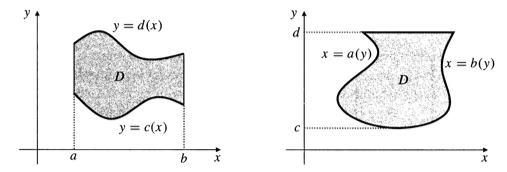
\includegraphics[scale=0.7]{image2.png}
\\
Les bords de la fonction pour y-simple sont $y=c(x)$ et $y=d(x)$.

Pour $x$-simple, c'est la même chose mais dans l'autre sens. Les bornes sont donc $x=a(y)$ et $x=b(y)$.
\begin{myrem}
$D$ peut être à la fois $x-$ et $y$-simple.
\end{myrem}
\begin{myrem}
Contre-exemple : Lorsqu'une des deux bornes n'est pas une fonction $y=d(x)$ ou $y=c(x)$, le domaine n'est pas y-simple. C'est la même chose pour x-simple.

\end{myrem}

\begin{myrem}
$D$ est ``régulier'' lorsqu'on peut trouver une union finie de domaines simples.


Par exemple, dans ce cas-ci, chacun des 4 sous-domaines est un domaine simple.\\
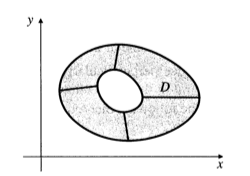
\includegraphics[scale=1]{image1.png}

\end{myrem}

\graphicspath{{CM2/}}
\part{Cours Magistral 2 -- Les intégrales}
\section{Utiliser/Généraliser Fubini}
Voire Figure 14.13(a)

Le domaine d'intégration représente un cercle sur le plan x-y. On définit $a$ et $b$, les deux limites du domaine sur l'axe des x (Voir Schéma (a) ci-dessous).

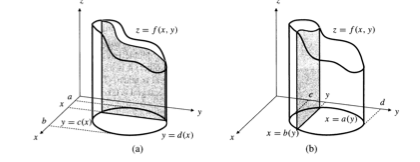
\includegraphics[scale=0.8]{image1.png}

Nous allons calculer l'intégrale d'abord selon y-simple ( Figure a ) puis selon x-simple ( Figure b ) puis comparer les résultats obtenus.
\paragraph{Y-simple}
On note $A(x)$ la surface de l'aire grisée de l'image $(a)$.
\[A(x)=\int_{c(x)}^{d(x)}f(x,y)dy\]
$\int_a^b A(x) \dif x$ est un petit élément de volume.

\[\int_a^b A(x) \dif x = \text{Volume de }S = \int_Df(x,y) \dif x \dif y\]

On pourra calculer le volume comme ceci :

\[ \iint_D f(x,y) \dif x \dif y = \int_a^b \int_{c(x)}^{d(x)} f(x,y)  \dif y \dif x = \int_a^b \dif x \int_{c(x)}^{d(x)} f(x,y) \dif y \]

On calcule d'abord l'intérieur de l'intégrale pour ensuite trouver l'extérieur (\textit{``Inner''} en anglais)
\begin{myrem}
``\emph{x}'' est considéré comme une constante dans l'intégrale ``intérieure''
\end{myrem}

\paragraph{X-ximple}

Voire Figure 14.13 (b)
\[\iint_D f(x,y) \dif x \dif y = \int_c^d\int_{a(y)}^{b(y)} \dif x f(x,y)\]
Nous avons le même résultat.\\
En pratique, on a souvent un domaine x-simple et y-simple ! Les deux calculs donneront le même résultats. Mais il y a presque toujours un sens de coupe qui est plus facile que l'autre. Voire exemple ci-dessous.

\subsection{Exemple 1}
\[ I=\iint_D xy \dif x \dif y \]
\begin{center}

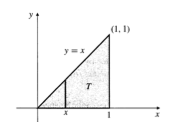
\includegraphics[scale=1]{image2.png}

\end{center}
Commençons par calculer selon \textbf{y-simple}
Les deux bords sont $y=0$ et $y=x$. Le domaine est y-simple. On se fixe un x et on fait la coupe verticalement (dans ce cas). Le point d'entrée est $y=0$ et le point de sortie est $y=x$.
\[I=\int_0^1 dx \int_0^x dy(xy)\]
Or on peut calculer l'intégrale interne
\[\int_0^x dy(xy) = \left[ x \frac{y^2}{2} \right]_0^x = \frac{x^3}{2}\]
On aura donc au final
\[I=\int_0^1\frac{x^3}{2} dx = \left[\frac{x^4}{8}\right]_0^1= \frac{1}{8}\]

On peut aussi calculer selon \textbf{x-simple}.
\\
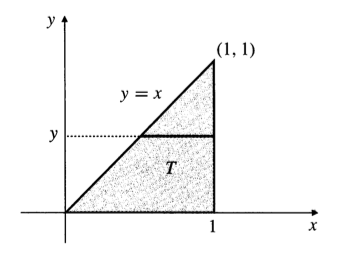
\includegraphics[scale=0.5]{image3}
\\

Le point d'entrée est $x=y$ et le point de sortie est $x=1$.
\[I=\int_0^1dy\int_y^1dx(xy)\]

Au sein de l'intégrale interne, y est constant.

\[\int_y^1dx(xy) = \frac{y}{2}(1-y^2)\]
Au final, on trouve l'intégrale.
\[I = \int_0^1 \frac{y}{2}(1-y^2) dy = 1/8\]

On a le même résultat si l'on considère le domaine x-simple ou y-simple!

\subsection{Exemple 2}
\[I = \int_0^1dx \int_{\sqrt{x}}^1 dy e^{y^3}\]

On voit que la variable x est entre 0 et 1 et que la variable y ne va pas plus haut que 1.
\\
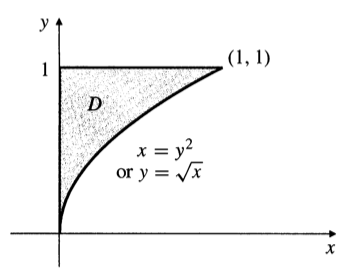
\includegraphics[scale=0.5]{image4.png}
\\

En regardant le domaine, on se rend compte qu'il est x-simple et y-simple !
\begin{itemize}

\item Les bords en x sont x=0 et $x=y^2$
\item Les bords en y sont $y=1$ et $y=\sqrt{x}$


\end{itemize}

\[I \overset{aussi}{=}\int_0^1dy \int_0^{y^2} dx e^{y^3}\]
\[\int_0^{y^2} dx e^{y^3} = e^{y^3} \int_0^{y^2} dx = e^{y^3} x \int_0^{y^2} = y^2 e^{y^3}\]
\[I=\int_0^1 y^2 e^{y^3} dy = \left[1/3 e ^{y^3}\right]_0^1  = \frac{e-1}{3}\]
Parce que
$y^2 e^{y^3} = \frac{d}{dy}(\frac{1}{3} e^{y^3})$

\section{Changement de variables}
Nous allons commencer par montrer un exemple pour prouver l'utilité du changement de variable pour ensuite passer au cas général.
\subsection{Exemple}
\[I=\int_D (1-x^2-y^2)\]
\begin{center}
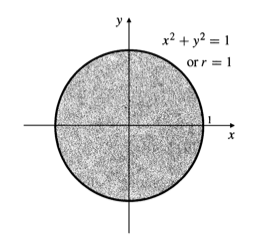
\includegraphics[scale=0.7]{image5.png}
\end{center}

 En y, le point d'entrée est $y=-\sqrt{1-x^2}$ et la sortie est  $y=\sqrt{1-x^2}$ ( pendant que x varie entre -1 et 1)

 \[I=\int_{-1}^1 dx \int_{-\sqrt{1-x^2}}^{\sqrt{1-x^2}} dy(1-x^2-y^2) \]

 \begin{myrem}
 $$\left\{
 \begin{array}{r}
 x=r\cos\Theta = \tilde{x}(r,\Theta)\\
 y=r \sin \Theta = \tilde{y}(r,\Theta)
 \end{array}
 \right.
 $$

 Exprimer f(x,y) en fonction de $(r,\Theta)$
 Calculer l'élément infinitésimale d'aire $dA$
 \end{myrem}

 On change donc de variables
 \[f(x,y)=1-x^2-y^2=f(x(r,\Theta),y(r,\Theta)) = g(r,\Theta)\]
 \[f(x,y) = 1-r^2\cos^2\Theta -r^2\sin^2\Theta = 1-r^2 = g(r,\Theta)\]
 \begin{center}

 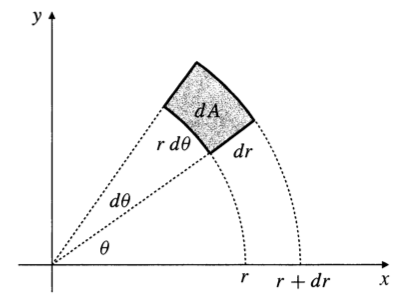
\includegraphics[scale=0.7]{image6.png}\\

 \end{center}
 Que vaut le petit élément $dA$ ? On considère que c'est un parralèllogramme.
 $dA\approx (rd\Theta)\times dr$
 \[dA = r dr d\Theta\]

 A présent, tout devient plus simple ! L'intégrale qui nous interesse devient donc.
 \[I=\int_S (1-r^2)r dr d\Theta\]
\begin{center}
 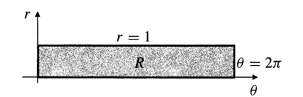
\includegraphics[scale=0.7]{image7.png}
\end{center}
 \[I=\int_0^{2\pi} d\Theta \int_0^1 dr r (1-r^2)\]
 \[I = \int_0^{2\pi} d \Theta \left(\frac{r^2}{2}-\frac{r^4}{4} \right) \text{évalué entre 1 et 0} = \frac{1}{4} \int_0^{2\pi} d \Theta = \pi/2 \]

\subsection{Cas général}

$$x=x(u,v)$$
$$y=y(u,v)$$
\begin{center}
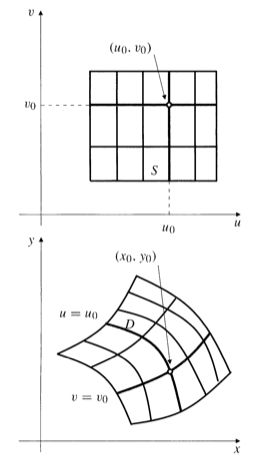
\includegraphics[scale=0.5]{image8.png}
\end{center}

On trace une courbe sur le deuxième graphique qui représente l'ensemble des points où $u=u_0$ est constant. Même chose pour $v=v_0$\\
Ce qui explique ce pavage "courbé". On apelle ça du \textit{"Mapping"}. Mais dans le cas d'un changement de variable, on veut que cette transformation soit bijective.\\

On peut donc trouver
$u=u(x,y)$
$v=v(x,y)$
\subsection{Jacobienne de la transformation}

Pour effectuer un changement de varibale, il faut calculer la jacobienne du changement de variable défini comme suit (Voir la suite pour savoir comment l'utiliser)

\[\tilde{J}=\frac{\partial ( u,v)}{\partial ( x,y) }\]

\[\tilde{J} =
\begin{vmatrix}
\frac{\partial u}{\partial x} &\frac{\partial u}{\partial y}\\
\frac{\partial v}{\partial x} &\frac{\partial v}{\partial y}\\
\end{vmatrix}
\]

On cherche donc la matrice $$J=\dfrac{1}{\tilde{J}}=\frac{\partial ( x,y) }{\partial ( u,v)}$$


$$J = \begin{vmatrix}
\frac{\partial x}{\partial u} &\frac{\partial y}{\partial u}\\
\frac{\partial x} {\partial v}&\frac{\partial y}{\partial v}
\end{vmatrix}$$


\[\iint_D f (x,y) \frac{dA}{dxdy}=\iint_S g(u,v) dA\]

\begin{center}
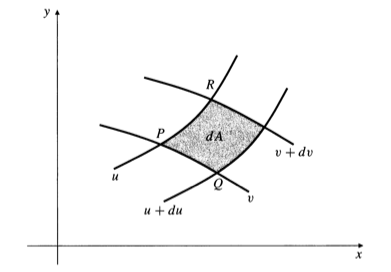
\includegraphics[scale=0.7]{image9.png}
\end{center}

\paragraph{P}
$$x(u,v)$$
$$y(u,v)$$
\paragraph{Q}
\[x(u+du,v)=x(u,v)+\frac{\partial x}{\partial u} du\]
\[y(u+du,v)=y(u,v)+\frac{\partial y}{\partial u} du\]
\paragraph{$\vec{PQ}$}

$$ \vec{PQ} = \left( \frac{\partial x}{\partial u} du\right) \hat{i} +\left( \frac{\partial y}{\partial u} du \right) \hat{j} $$
\paragraph{$\vec{PR}$}
$$\vec{PR} = \left(\frac{\partial x}{\partial v} dv \right) \hat{i} + \left( \frac{\partial y}{\partial v} dv \right) \hat j $$

Toutes les $ \frac{\partial .}{\partial .} $ sont calculées en $(u,v)$
\[dA \approx || \vec{PQ} \times \vec{PR}|| \]

\[ ||det
\begin{vmatrix}
\hat i & \hat{j} & \hat{k}\\
\left(\frac{\partial x}{\partial u} du) \right) & \left(\frac{\partial y}{\partial u} du) \right) & 0 \\
\left(\frac{\partial x}{\partial v} dv) \right) & \left(\frac{\partial y}{\partial v} dv) \right) & 0

\end{vmatrix}||
\]

\[=||\left(\frac{\partial x}{\partial u} \frac{\partial y}{\partial v} - \frac{\partial x}{\partial v} \frac{\partial y}{\partial u}\right) du dv \hat{k} ||\]
\[= dA = |J|dudv\]

\fbox{
\begin{minipage}{10cm}

\textbf{Formule à connaître \# 1}

Cette formule est primordiale lors du calcul d'une intégrale avec un changement de variables.

\[\iint_D f(x,y)dxdy = \iint_S g(u,v) \left| \frac{\partial (x,y)}{\partial (u,v)} \right| dudv\]

$$x=x(u,v) \text{ et }  y = (u,v)$$

$$ D \longleftrightarrow S $$ Il doit y avoir une bijection entre les variables de départ et les varibles de fin.\\
\textit{La valeure absolue nous offre la liberté de choisir l'ordre des lignes et des collones de la jacobienne.}
\end{minipage}
}

\subparagraph{Exemple}



$$x=x(u,v)=x(r,\Theta)=r\cos(\Theta)$$
$$y=y(u,v)=y(r,\Theta)=r\cos(\Theta)$$





\[
\frac{\partial (x,y)}{\partial (r, \Theta)} =
\begin{vmatrix}
\frac{\partial x}{\partial r}& \frac{\partial x}{\partial \Theta}\\
\frac{\partial y}{\partial r}& \frac{\partial y}{\partial \Theta}
\end{vmatrix}
\]

$$\begin{vmatrix}
\cos\Theta & -r\sin\Theta\\
\sin\Theta & R\cos\Theta
\end{vmatrix}$$
\[=r\cos^2\Theta +r\sin^2\Theta = r > 0\]
$$dA = |J|dudv \overset{ici}{=}r dr d\Theta $$

\begin{myrem}

Lire la page 816 ex 11
\end{myrem}

\subsection{Changement de variables $ \iiint_D $}
$$
\left\{
\begin{array}{l}
x=x(u,v,w)\\
y=y(u,v,w)\\
z=z(u,v,w)\\
\end{array}
\right.
$$

$D \longleftrightarrow S $

\[\int_D f = \int_S f (x(u,v,w),y(u,v,w),z(u,v,w) dV\]
\[f (x(u,v,w),y(u,v,w),z(u,v,w)) = g(u,v,w)\]

\[dV=\left|\frac{\partial(x,y,z)}{\partial(u,v,w)}\right|dudvdw\]



\subsubsection{Coordonnées sphériques}

Le passage aux coordonnées sphérique est un changement de variable $\iiint_D$
\begin{myrem}

Voire les images 14.45,14.47,14.50,14.52
\begin{figure}


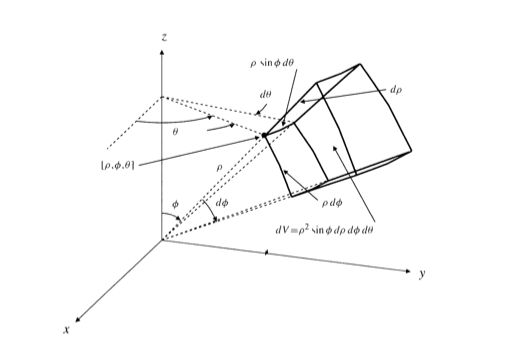
\includegraphics[scale=0.5]{image10.png}
\caption{14.45}
\end{figure}

\begin{figure}
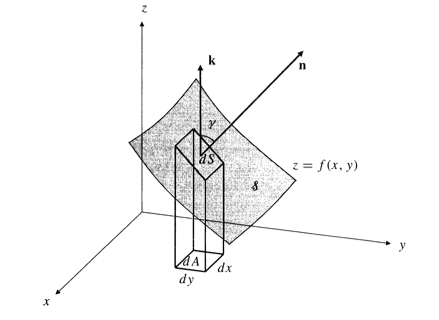
\includegraphics[scale=0.5]{image11.png}
\caption{14.47}
\end{figure}

\begin{figure}
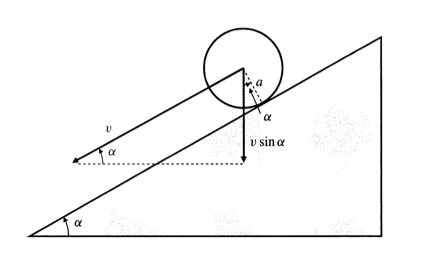
\includegraphics[scale=0.5]{image12.png}
\caption{14.50}
\end{figure}


\end{myrem}
$$
\left\{
\begin{array}{l}

x=g\sin\phi cos\Theta\\
y=g\sin\phi sin\Theta\\
z=g\cos\Theta

\end{array}
\right.
$$

est un exemple de changement de variable sphérique.
\[dV=g^2\sin\phi dgd\phi d\Theta \]

Faire l'exerice F14.42(b) !



\section{Moyenne d'une fonction}
$f\text{D} \subset \Re ^n$ et on a aussi $\overline{f} = $ moyenne de f constante sur D

\[\int_D \overline{f} \eqdef \int_D f = \overline{f}\int_D 1 = \overline{f}\text{Vol(D)}\]

$$\Rightarrow\ \overline{f} = \frac{\int f}{\text{Vol(D)}}$$
\begin{itemize}
\item \textbf{1D} $\overline{f}=\frac{1}{L}\int f$
\item \textbf{2D} $\overline{f}=A^{-1}\iint f$
\item \textbf{3D} $\overline{f} = V^{-1}\iiint f$
\end{itemize}

\graphicspath{{CM3/}}
\part{Cours Magistral 3 -- Les intégrales}
\section{Introduction}

\begin{center}
\begin{tabular}{l l}

$\int_D f$ &  $f: D\to \mathbb{R}$ \\
&$D$ borné dans $\mathbb{R}^n$
\end{tabular}

\end{center}


\[
\left\{
\begin{array}{l}
D=[a,b]\subset\mathbb{R}\\
D=S\subset\mathbb{R}^2\\
D=V\subset\mathbb{R}^3\\
\end{array}
\right.
\]



\[\int_D 1 = \text{"Volume" de D (longueur de [a,b], aire de S, volume de V)}\]

avec $f\equiv1$
\[ f=\text{densité de matière répartie sur D (par unité de Volume)} \]
\[\int_D f = \text{masse totale répartie dans D = masse de D}\]

Dans ce cours, nous allons voir comment calculer
\begin{itemize}
\item la longueur d'une courbe;
\item l'aire d'une surface
\end{itemize}

\section{Intégrale de ligne d'un champ scalaire}

Voir~\cite{adams2013calculus} p.~875 section~15.3.

Un champ scalaire est une fonction qui associe à chaque point de l'espace ou d'un plan (on parle alors d'un champ scalaire plan) un scalaire. La température dans l'espace à un moment donné est un champ scalaire. On peut également ajouter une composante temporelle (en effet, la température dans l'espace change en fonction du temps). Le champ scalaire sera donc une fonction de $\mathbb{R}^4 \to \mathbb{R} $

\[r=r(t)=x(t)\xunit+ y(t)\yunit+z(t)\zunit = (x(t),y(t),z(t))\]

avec \[a\leq t\leq b\] et où r est le vecteur position d'un point de la courbe C dans le repère ($\xunit,\yunit, \zunit$)

\textbf{Représentation paramétrique de C :}

Droite $d$ scalaire $f(x,y,z)$ donnée $\to \int_C f$
\[a=t_0<t_1<t_2<\dots<t_n=b\]

On va donc calculer les points
\[r_i = r(t_i)\]

Dans chaque segment arbitrairement choisi
\[t_i^*\in[t_{i-1},t_i]\]

\[r_i^*=r(t_i^*)=(x_i^*,y_i^*,z_i^*)\]

Maintenant, nous allons former les sommes de Riemann appelées $S_n$
\[S_n=\sum_{i=1}^nf(x_i^*,y_i^*,z_i^*)\norm{\Delta r_i}\]

Passage à la limite $n\to\infty$; max$\abs{\Delta r_i}\to 0$

\[I=\int_C f = \int_C f (x,y,z)\dif S\]

où $\dif S$ est la longueur d'arc infinitésimale.

\begin{mytheo}
Si (condition suffisante) C est de classe $C^1$ et est continue sur C, alors $\int_C f$ existe\\
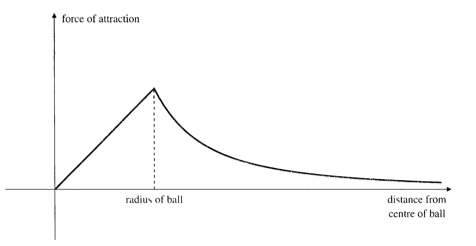
\includegraphics[scale=0.5]{exemple1.png}\\
La fonction n'est pas de classe $C^1$
\end{mytheo}

\begin{myrem}

$f\equiv1$
\[\int_C 1 = \int_C \dif S = \text{longueur de la courbe entre le point de départ et le point d'arrivée}\]
\end{myrem}

\begin{myrem}
Si $f$ est une densité de matière par unité de longueur, alors $\int_C f  = \text{masse totale répartie le long de }C$
\end{myrem}

On reprend la formule
\[S_n=\sum_{i=1}^nf(x_i^*,y_i^*,z_i^*)\norm{\Delta r_i}\]
 et on pose \[\norm{\Delta r_i }=\frac{1}{\Delta t_i}\norm{\Delta r_i} \Delta t_i\]


 \[\lim_{\Delta t_i \to 0} \frac{\Delta r_i}{\Delta t_i} = \frac{\dif r}{\dif t}(t=t_i)\]

\fbox{
\begin{minipage}{10cm}


\textbf{Formule à connaître \# 2 }\\
 \textit{Règle de calcul}
 \[\int_C f = \int_C f (x,y,z)\dif S = \int_a^b f(r(t))\norm{\frac{dr}{dt}} \dif t\]
 $f(r(t))$
 évalué le long de la courbe $f(x(t),y(t),z(t))$
 
 Cette formule sert à calculer l'intégrale d'un champ scalaire sur une ligne.
 \end{minipage}
 }
\\

 Exemple :

 Demi-cercle centré à l'origine de rayon $a$. Le point $(x,y)$ se trouve à une amplitude $t$ par rapport au point $(a,0)$

 \[\int_C y \dif S\]

 \begin{itemize}

 \item
 \[r(t) = (a \cos t ) \xunit + ( a \sin t )\yunit +0k\]
avec $ 0\leq t \leq r $ et $a \cos t =x(t)$ et $a \sin t = y(t)$ et $t$ croissant $(\dif t>0)$

Dès qu'on a choisi une représentation, on a choisi un sens de parcours.
\item
\[\frac{\dif r}{\dif t}=(-a\sin t )\xunit + (a \cos t ) \yunit\]

 où $(-a\sin t ) = \frac{\dif x(t)}{\dif t}(t)$ et $(a\cos t ) = \frac{\dif y(t)}{\dif t}(t)$

\item \[\norm{\frac{\dif r}{\dif t}}=a\]
\item \[I = \int_C y \dif s = \int_0^{\pi} f(r(t))a\dif t\]

$f(r(t))$ est calculé le long de la courbe $= y$ sur la courbe
\[I=\int_0^2 a \sin{t} \, a \dif t = -a^2 \cos t \Big \rvert^\pi_0 =2a^2\]
 \end{itemize}

Nous pouvons choisir une autre représentation paramétrique de la courbe C et nous obtiendrons le même résultat.

\[x^2+y^2 = a^2\]

On choisit $x$ comme paramètre.

Dans le dessin d'un demi-cercle de rayon $a$

\[x \in [-a;a]\]
\[y=\sqrt{a^2-x^2}\]
\[r(t) = (x)\xunit + \sqrt{a^2-x^2} \yunit\]

Quand on va de $-a$ à $a$, on parcourt la courbe mais dans l'autre sens. On a choisi une autre représentation paramétrique. Faire l'exercice à la page 859 et on trouvera le même résultat, c'est-à-dire $2a^2$

On peut donc conclure que

$I=\int_C f \dif S$ ne dépend pas du choix de la représentation paramétrique de C. Et c'est normal parce que pour un problème physique, la masse d'un objet ne peut pas dépendre de la méthode mathématique que l'on utilise pour la calculer.

\section{Intégrale d'un champ scalaire sur une surface}
Voir~\cite{adams2013calculus}, p.~887 section~15.5
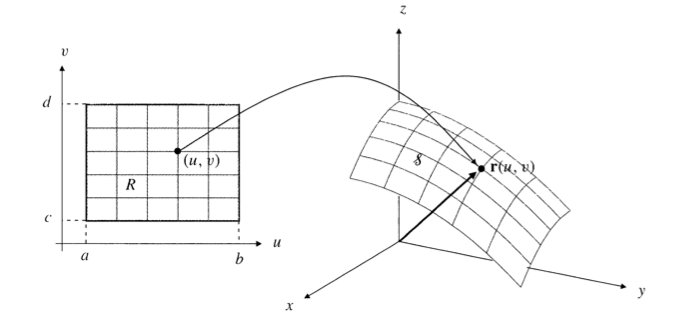
\includegraphics[scale=0.5]{courbe1.png}%p832
\\
Il y a un mapping $r(u,v)$ de $\mathbb{R}$ dans $S$. À partir du quadrillage initial, on obtient des courbes correspondantes.


\[\vec r(u,v)=x(u,v)\xunit +y(u,v)\yunit +z(u,v)\zunit\]

avec $(u,v)\in \mathbb{R}$

On peut considérer que le bord de $R$ est projeté sur les bords de $S$. Mais, ici, on ne demande pas que l'application (le mapping) soit \emph{bijective}.

Exemple : \[r(u,v) = (a \cos u \sin v) \xunit + (a \cos u \sin v) \yunit +(a \cos v) \zunit\]

avec $a \cos u \sin v = x(u,v)$, $(a \cos u \sin v)=y(u,v)$ et $(a \cos v) =z(u,v)$

\[
R=
\left\{
\begin{array}{c}
0\leq u \leq 2 \pi ; 0\leq v\leq \pi /2\\

a = \textbf{cst} > 0
\end{array}
\right\}
\]

C'est une demi-sphère d'équation

\[x^2+y^2+z^2 = a^2\]

Domaine :
$u$ va de $0$ à $2\pi$ et $v$ va de 0 à $\pi /2$

Par le mapping, un point du rectangle du domaine va vers un point de la demi-sphère.

Tous les points sont transformés en \[\vec r (u,\pi/2 ) = (a \cos u  )\xunit + (a \sin u )\yunit \] avec $0\leq u \leq 2 \pi $

\[v=0 \to r(u,0) = 0 \xunit + 0 \yunit + a \zunit\] autrement dit, le point (0,0,a)


Le bord de la demi-sphère n'est défini que par une partie du bord du rectangle (quand $v=\pi/2$ et que $u$ varie de $0$ à $2\pi$).
Il n'y a pas de bijection mais ce n'est pas grave.


\[\int_S f(x,y,z)\dif S\]

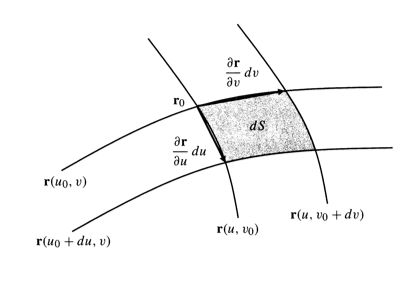
\includegraphics[scale=0.5]{courbe2.png}

On a trouvé ce graphique en partant d'un rectangle où $u$ va de $u_0$ à $u_0 + \dif u$ et $v$ va de $v_0$ à $v_0+\dif v$

Pour déterminer une telle intégrale, nous avons besoin de la somme de Riemann.

\[S_n = \sum_{i=1}^nf(x_i^*,y_i^*,z_i^*) \Delta S_i\]

Dans la formule, $\int_S f(x,y,z)\dif S$,

\[f(x,y,z)=f(r(u,v))\] Mais on ne connait pas la valeur de $dS$

Voir le schéma ci-dessus.

$\frac{\partial \vec r }{\partial u } \text{ et } \frac{\partial \vec r }{\partial v }$ sont évaluées en $(u_0,v_0)$

\[\dif S = \norm{\frac{\partial r }{\partial u } \times \frac{\partial r }{\partial v }} \dif u \dif v\]

La signification géométrique de $ \frac{\partial r }{\partial u } \times \frac{\partial r }{\partial v }$ est le vecteur tangent au point $r_0$.

Il n'y a plus qu'à calculer.

\[\frac{\partial r }{\partial u} =
\left( \frac{\partial x}{\partial u}(u,v)\right)\xunit +
\left( \frac{\partial y}{\partial u}(u,v)\right)\yunit +
\left(\frac{\partial z}{\partial u}(u,v)\right)\zunit
\]


\fbox{
\begin{minipage}{10cm}

\textbf{Formule à connaître \#3}
\[
\frac{\partial (F,G)}{\partial (x, y)} =
\begin{vmatrix}
\frac{\partial F}{\partial x}& \frac{\partial F}{\partial y}\\
\frac{\partial G}{\partial x}& \frac{\partial G}{\partial y}
\end{vmatrix}
=\frac{\partial F}{\partial x} \frac{\partial G}{\partial y}- \frac{\partial F}{\partial y}\frac{\partial G}{\partial x}
\]

\[dS=\sqrt{\left(
\left( \frac{\partial(y,z) }{\partial (u,v)}\right)^2 +
\left( \frac{\partial(z,x) }{\partial (u,v)}\right)^2 +
\left( \frac{\partial(x,y) }{\partial (u,v)}\right)^2
\right)}
\dif u\dif v\]


\[\int_S f = \int _S f(x,y,z) \dif S = \iint_R f(x(u,v),y(u,v),z(u,v)) \dif S\]

Avec cette formule, nous pouvons calculer l'intégrale d'un champ scalaire sur une surface.
\end{minipage}
}

Cas particulier : $f\equiv 1 : \int_S 1 = \int_S \dif S = \text{aire de S}$

\[f \equiv 1 = \int_C 1 = \int_C \dif S = \text{longueur de la courbe}\]


\textbf{Exemple }: Un graphique dont le domaine représente une surface D et dont l'aire représente une surface $S=$ graphe de $g$.


 $g(x,y) : D\subset\mathbb{R}^2 \to \mathbb{R}$ donné


Comment calculer $\int_Sf \dif S$ ? Il faut trouver la représentation paramétrique par exemple
$x=u; y=v; z=g(u,v)$

$\forall (u,v) \in D $


\[\Rightarrow r (u,v) = (u)\xunit+(v)\yunit+(g(u,v))\zunit\]

On peut lancer l'algorithme.

On cherche d'abord tous les déterminants.

\[\frac{\partial (y,z)}{\partial (u,v)} =
\begin{vmatrix}
\frac{\partial y}{\partial u}& \frac{\partial y}{\partial v}\\
\frac{\partial z}{\partial u}& \frac{\partial z}{\partial v}
\end{vmatrix} =
\begin{vmatrix}
0&1\\
\frac{\partial g}{\partial u}&\frac{\partial g}{\partial v}
\end{vmatrix}
= \frac{-\partial g}{\partial u}\]
Un autre,
\[\frac{\partial (z,x)}{\partial (u,v)} = \frac{-\partial g}{\partial v}\]
et le dernier,
\[\frac{\partial (x,y)}{\partial (u,v)} = 1\]

On calcule

\[\int_S f = \iint_D f(x,y,g(x,y)) \dif S = \iint_D f(u,v,g(u,v))\sqrt{1+(\frac{\partial g}{\partial u})^2 +(\frac{\partial g}{\partial V})^2 } \dif u\dif v
\]

avec $f$ évaluée sur la surface.

\section{Intégrale de la composante tangentielle d'un champ de vecteur $F(x,y,z)$ le long d'une courbe $C$}

Voir~\cite{adams2013calculus}, p.~879, section~15.4\\


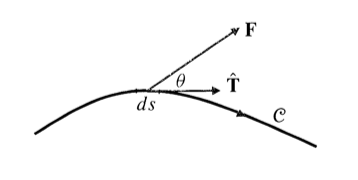
\includegraphics[scale=0.5]{vec1.png}\\

\[\dif W = \vec F\cdot \vec \dif r = F\cdot \hat{T} \dif S\]
et $\hat{T}$ est la tangente unitaire à $C=\frac{\dif r}{\dif t}\frac{1}{\norm{\frac{\dif r}{\dif t}}}$. C'est une dérivée partielle.

(Voir~\cite{adams2013calculus} section~11.4 ou la partie du cours donnée par M. Glineur).

\[\dif W = \norm{F} \cos \Theta \dif S\]
On souhaite calculer

\[\int_{A\to B} \dif W = \text{travail total exercé par la force F sur la particule le long de C}\]


\[\vv{F}=F_1 \xunit + F_2 \yunit +F_3 \zunit\]
\[\vv{F} = \vv{F}(x,y,z)\]

On cherche
\[\int_C\vv{F}\cdot \hat T \dif S\]

et $\cdot$ est un produit scalaire. Le résultat est un \emph{scalaire}.

\[= \int_C F\cdot \dif r = \int_C \vv{F}\]

En fait, c'est l'intégrale de la composante tangentielle du vecteur.

$\int_C F\cdot \hat T \dif S$ est une intégrale de type connu. Elle peut être écrite sous la forme $\int_C f \dif S$ où $f=F \cdot \hat{T}$

L'intégrale dans un sens est l'opposé de l'intégrale dans l'autre sens.

\[I^{\ominus} = -I^{\oplus}\]



\fbox{
\begin{minipage}{10cm}
\textbf{Formule à connaître \# 4}
\[r(t)= x(t)\xunit+y(t)\yunit+z(t)\zunit\]
$a\leq t\leq b$

$$\int_C F = \int_C F\cdot \dif r = \int_C ( F \cdot \frac{\dif r}{\dif t}) \dif t $$
\[= \int_a^b \left[F_1( x(t),y(t),z(t)) \frac{\dif x(t)}{\dif t}+
F_2( x(t),y(t),z(t)) \frac{\dif y(t)}{\dif t}+\right.\]
\[\left.
F_3 (x(t),y(t),z(t)) \frac{\dif z(t)}{\dif t}\right]\cdot dt\]

Cette formule nous montre comment calculer l'intégrale d'un champ vectoriel sur une ligne.
\end{minipage}
}
\\
\\
\textbf{Exemple 1} :
Un champ vectoriel qui a pour équation :
\[F(x,y)=(y^2)\xunit+(2xy)\yunit\]

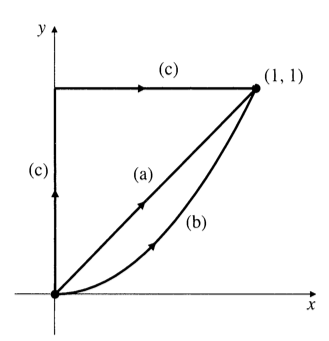
\includegraphics[scale=0.6]{courbe3.png}\\
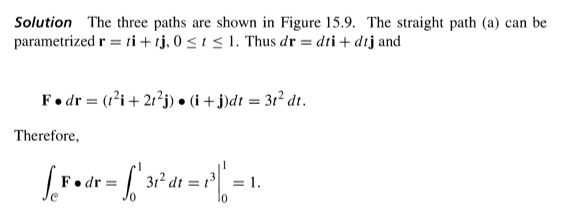
\includegraphics[scale=0.6]{resolu1.png}

Sur les deux autres chemin, on va toujours trouver 1. Il y a beaucoup de chance que cette force soit conservative mais c'est possible que non. Pour en être sur, il faudrait calculer par tous les chemins possibles et voir si on a toujours le même résultat. Pour ça, on applique le Théorème de Poincaré (cf. CM4). D'un point de vue mathématique, on se demande si c'est un champ de vecteur conservatif. Le Théorème de Poincaré nous permettra de le déterminer.

\begin{mytheo}[Théorème de Poincaré]
Voir plus tard.
\end{mytheo}
\textbf{Exemple 2 }: \[F=y\xunit-x\yunit\]

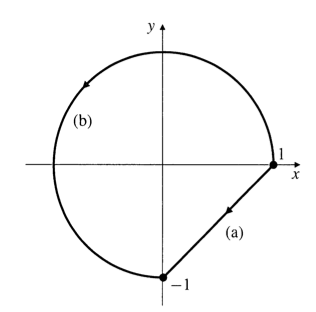
\includegraphics[scale=0.7]{resolu2.png}
\[\int_C F \cdot \dif r\]
\[
\left\{
\begin{array}{l}
I(a)=1\\
I(b)=-3\pi/2
\end{array}
\right.
\]

Avec les deux chemins, on ne trouve pas le même résultat. F n'est donc évidemment pas conservative.

\graphicspath{{CM4/}}
\part{Cours Magistral 4 -- Les intégrales}
\section{Rappel}

Nous considérons deux champs de vecteurs bidimensionnels (également appelés champs vectoriels plans)
\[
\left\{
\begin{array}{c}
F=y^2\xunit+2xy\yunit\\
F = y\xunit-x\yunit
\end{array}
\right.
\]

\[\int_C F\cdot \dif r \]

\section{Intégrale le long d'un chemin}
Cette section se réfère à la section~15.4 de~\cite{adams2013calculus}

\subsection{Champ de vecteurs conservatif ou dérivant d'un potentiel scalaire}

\[F:(F_1,F_2,...F_n)\text{dans } \mathbb{R}^n\]

\[F_i=F_i(x_1,x_2,...,x_n)\]

$F$ est conservatif ssi il existe un champ scalaire.

\[F=\text{grad}\Phi = \nabla \Phi\]
\[F_i=\frac{\partial \Phi}{\partial x_i}\]
\begin{myrem}
\[F=-\nabla U = \nabla (- U ) = \nabla ( \Phi ) \]
\end{myrem}

\begin{myrem}{(Forme) différentielle exacte}

Pas dans le livre !

\[F_1 \dif x +F_2 \dif y + F_3 \dif z \] est une différentielle exacte ssi\[F_1 \dif x +F_2 \dif y + F_3 \dif z  = \dif\Phi\]
ssi
\[\frac{\partial \Phi}{\partial x_i} = F_i\]
\end{myrem}

Les composantes d'un champ de vecteurs conduisent à écrire une différentielle exacte. Notion utilisée en thermodynamique.

Si $F$ est la dérivée d'un potentiel scalaire $\Phi$, alors $\forall$ C allant de $P_0$ à $P_1$ fixés,

\[\int_C F\cdot \dif r = \Phi ( P_1 ) - \Phi ( P_0) \]

On peut écrire
\[\int_C \nabla \Phi \cdot \dif r =  \Phi ( P_1 ) - \Phi ( P_0) \]

C'est une généralisation de $\Phi = \int F $ et $\Phi ' = F $

\[F\bullet \dif r = \left( \frac{\partial \Phi }{\partial x} \xunit + \frac{\partial \Phi }{\partial y} \yunit +\frac{\partial \Phi }{\partial z} \zunit \right)\cdot (\dif x \xunit + \dif y \yunit + \dif z \zunit)\]

\[=\frac{\partial \Phi}{\partial x}\dif x + \frac{\partial \Phi}{\partial y}\dif y +\frac{\partial \Phi}{\partial z}\dif z = \dif \Phi\]

On trouve donc

\[\int_C F\cdot \dif r = \int_C ( \nabla \Phi \cdot \frac{\dif r}{\dif t} ) \dif t \]

avec \[( \nabla \Phi \cdot \frac{\dif r}{\dif t} )= \frac{\dif \Phi}{\dif t}((r(t))\]

Donc,

\[\int_C F\cdot \dif r = \Phi ( P_1 ) - \Phi ( P_0) \]

Attention, c'est une simple implication !

Si $F$ est conservatif, alors
on peut prendre un chemin fermé, c'est à dire $P_0 = P_1$. On aura donc

\[\oint _C F\cdot \dif r = 0\]

où $ \oint $ est l'intégrale fermée.

À présent, on considère deux chemins différents pour aller de $P_0$ à $P_1$. Le premier chemin est $C_1$ et le deuxième est $C_2$.

On calcule le chemin sur $C = C_1-C_2$

\[\oint _C F\cdot \dif r = 0\]

On aura donc \[\int_C F = \int_{C_1} F - \int_{C_2} F = 0\]

Donc, on trouve
\[\int_{C_1} F = \int_{C_2} F \]

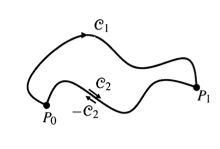
\includegraphics[scale=1]{image3.png}

Un dernier point :

Si l'on calcule tous les chemins possibles entre $P_1$ et $P_0$ et qu'il y a indépendance de chemin, peut-on conclure que le champ de vecteur $F$ est conservatif ?

La réponse est : \og \c Ca dépend\fg{}.

Mais la réponse est oui dans le cas où F est défini sur un domaine $D\subset \mathbb{R}^n$ ouvert et connexe.
\begin{mydef}

Un domaine est connexe si quel que soit le couple de points $P_0$ et $P_1$, on peut trouver un chemin pour relier les deux points.
\end{mydef}


Un exemple de domaine qui n'est pas connexe : \\
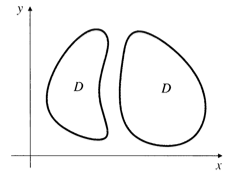
\includegraphics[scale=1]{image1.png}
\\
Un exemple de domaine connexe :
\\
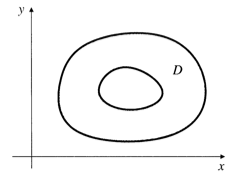
\includegraphics[scale=1]{image2.png}

\subsection{Démonstration constructive}

(C'est une démonstration qui explique comment calculer en plus de démontrer)

On considère dans l'espace de $\mathbb{R}^3$, un point $P$ de coordonnées $P_0 = (x_0,y_0,z_0) $  et $P = (x,y,z)$

\[P_0, P \in D \text{ ouvert et connexe }\]

On définit $\Phi$ tel que

\[\Phi (x,y,z ) =\int_C F\cdot \dif r \]
où C est une courbe reliant $P_0$ à $P$.

On a utilisé le fait que le domaine est connexe et qu'il y a indépendance des chemins.

On va montrer que \[\nabla \Phi = F \Longleftrightarrow F \text{ conserv.} \]

\[\frac{\partial \Phi}{\partial x} \overset{?}{=} F_1 (x,y,z) \]

On peut trouver un point $P' = ( x_1,y,z)$ tel que $x_1 < x$ est dans le domaine. On est certain de le trouver comme le domaine est ouvert.

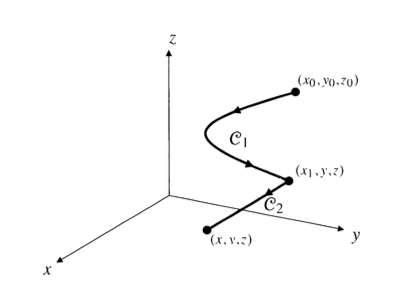
\includegraphics[scale=0.7]{image4.png}

\[C=C_1+C_2\]
\[\Phi (x,y,z) = \int_{C_1} F + \int_{C_2} F\]

On trouve que $\int_{C_1} F$ ne dépend pas de x. Donc $\frac{\partial I_1}{\partial x }=0$

\[x_1\leq t \leq x \]
\[r(t) = t \xunit +y\yunit + z \zunit \]
\[\dif r = \frac{\dif r}{\dif t}\dif t = (\dif t)\xunit\]

On a donc

\[I_C = \int_{x_1}^x (F\cdot i)dt = \int_{x_1}^x F_1 \dif t\] avec $F_1 = F_1 ( t,y,z )$

On vient de montrer que

\[\frac{\partial I_2	}{\partial x} = F_1 = \frac{\partial \Phi}{\partial x}\]


\begin{mytheo}

\textbf{À connaître}

Soit $D$ ouvert connexe de $\mathbb{R}^n$ et $F$ champ de vecteurs défini dans $D$. Il y a \textbf{équivalence} des trois énoncés suivants.

\begin{itemize}
\item $F$ est conservatif sur $D$, c'est-à-dire qu'il existe un potentiel scalaire $\Phi$ tel que $F=\nabla \Phi $ dans $D$;
\item $\oint_C F =0 \forall $ courbe fermée de $D$;
\item $\forall P_0,P_1$ dans $D$, $\forall$ chemin $C$ reliant $P_0$ et $P_1$ dans $D$,
\end{itemize}
\[\int_C D \text{ a une valeure identique ( indépendance de chemin ) }\]

\end{mytheo}

\begin{mytheo}[Théorème de Poincaré]

Connaissant $F$, puis-je facilement décider si $F$ est (ou non) conservative ? (Sans essayer de trouver un potentiel $\Phi$ ni essayer de trouver une infinité de chemins).

Nous verrons plus loin que pour D simplement connexe, on peut ajouter un 4\ieme{} énoncé.

$$\frac{\partial F_i}{\partial x_j} = \frac{\partial F_j}{\partial x_i}$$

Ce théorème est applicable uniquement si le domaine est simplement connexe.
\end{mytheo}

\begin{mydef}
$D$ simplement connexe ssi connexe et toute courbe fermée qui ne s'intersecte pas peut être  transformée continument en un point de $D$ sans quitter $D$.
\end{mydef}

Par exemple :

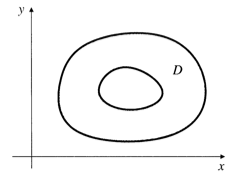
\includegraphics[scale=0.7]{image2.png}\\
n'est pas simplement connexe.
La fonction $ \Phi =xy^2 $  est le potentiel $F=y^2\xunit +2xy\yunit$ (par définition, c'est un champ de vecteur conservatif.)

$F= y\xunit-x\yunit$, calculons, $\frac{\partial F_1}{\partial y} = 1 \neq \frac{\partial F_2}{\partial x} = -1$. En effet, pour qu'un champ de vecteurs soit conservatif, il faut que ces deux dérivées partielles soient égales.

Pour utiliser le Théorème de Poincaré, on doit d'abord vérifier que les hypothèses sont vérifiées.

\section{Le flux d'un champ de vecteur à travers une surface}

cf.~\cite{adams2013calculus} section~15.6

C'est une intégrale de surface de la composante normale à une surface d'un champ de vecteurs.

\subsection{Introduction}
 Surface orientée\\
 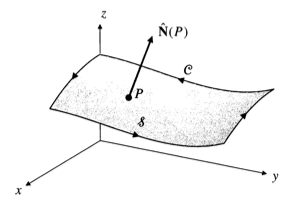
\includegraphics[scale=0.6]{image5.png}

 Le côté positif de la surface est le côté du vecteur normal tandis que le côté négatif, c'est l'autre.

 Par convention, l'orientation d'une surface induit une orientation particulière des bords de la surface (s'ils existent).

 La règle est la suivante : on se met sur la face positive de $S$ et on marche le long du bord $C$ en laissant $S$ à gauche, ce qui définit l'orientation positive de $C$.

 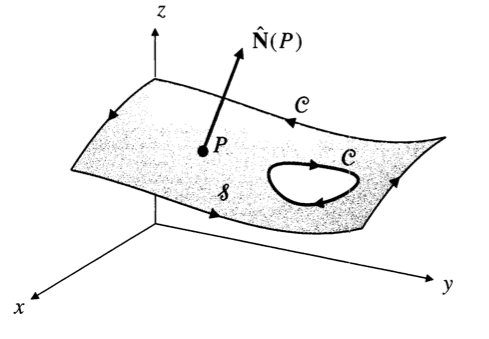
\includegraphics[scale=0.7]{image6.png}
 \\

 La face positive est au-dessus et la face négative est en-dessous. Par convention, les flèches représentent le sens de parcours positif.

 Voir ces exemples :

 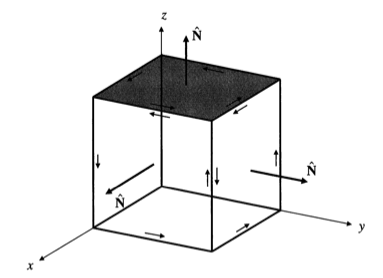
\includegraphics[scale=0.6]{image7.png}\\
 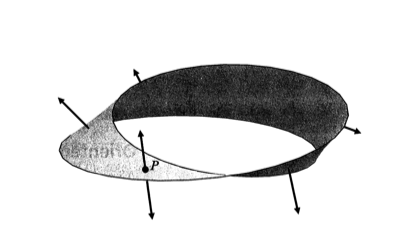
\includegraphics[scale=0.6]{image8.png}

 \subsection{Flux d'un champ vectoriel à travers une surface}

 On souhaite connaître la vitesse d'un cours d'eau à un endroit donné. On va placer une surface S fictive.\\

 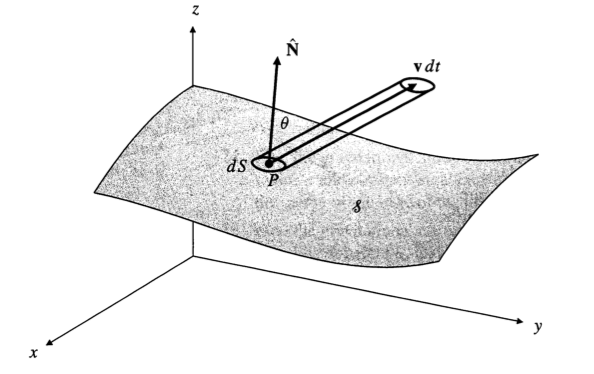
\includegraphics[scale=0.5]{image9.png} % Image 15.29
\\ On cherche le volume du cylindre. On pose $\rho \equiv 1$

 \[Vol = \norm{V}\dif t \cos \Theta \dif S\]

 avec $\norm{V}\dif t \cos \Theta = V\cdot \hat N \dif S$


 Par unité de temps, la quantité de fluide qui passe à travers $\dif S$ est donc \[V(P) \cdot \hat N(P) \dif S\]

 \[\int_S \text{flux } \dif S = \text{ flux total de matière à travers S.}\]

 \begin{mydef}
 Le flux d'un champ de vecteurs $F$ à travers une surface orientée S est donné par\[\int_S F \cdot \hat N \dif S = \int_S F \cdot \vv{\dif S}\]

 et $F \cdot \hat N$ est la composante normale à $S$ de $F$ avec $\vv{\dif S} = \hat N \dif S$ élément de surface vectoriel.

 Notation : $\int_C F$
 \end{mydef}

\begin{myrem}

$S$ fermée (sphère) :  $ \oiint_S F\cdot \dif S$

\[\oint F\cdot \dif r\]

\end{myrem}

Exemple : $F = (x) \xunit + (y) \yunit+(z) \zunit$

Flux sortant du cylindre
\[\left\{
\begin{array}{c}
F=y^2\xunit+2xyjx^2+y^2\leqslant a^2 \\ % FIXME je ne sais vraiment pas ce qui était sensé être écrit
-h\leqslant z \leqslant h
\end{array}
\right.\]


La surface totale $S$ : dessus + dessous + coté.

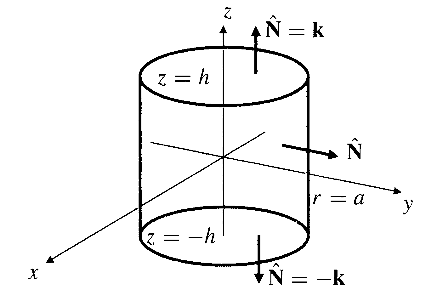
\includegraphics[scale=0.5]{image10.png}

\[\int_S F\cdot \dif S = \Sigma\text{flux}\]

On calcule sur chacune des faces.

\begin{enumerate}
  \item
    $z = +h$; $\hat N = \zunit$ et  $\dif S= r\dif\Theta \dif r$

    \[\int_{top}F\cdot \hat N \dif S = \int_O^{2\pi} d\Theta \int_0^a h r \dif r = \pi a^2 h\]

  \item $z = +h$; $\hat N = -k \Rightarrow =\pi a^2 h $

  \item coordonnées cylindriques

    \[-h \leq z\leq h \] et aussi
    \[0\leq \Theta \leq 2 \pi\]

    $\dif S = a\dif \Theta \dif z$

    \[\vec{F} = (a\cos\Theta ) \xunit +(a\sin\Theta ) \yunit + z \zunit  \]

    \[\hat N = (\cos\Theta ) \xunit +a\sin\Theta ) \yunit\Leftrightarrow \vec F \hat N \dif S = a^2\dif \Theta \dif z\]
    \[\int_0^{2\pi} \dif \Theta \int_{-h}^{+h} a^2 \dif z = 4\pi a^2 h\]

\end{enumerate}

Le flux total vaut donc la somme de (1), (2) et (3) $= 6 \pi a^2 h $

\fbox{
\begin{minipage}{10cm}
\textbf{Formule à connaître \# 5}

Règle de calcul


$r(u,v)$ de $S$ avec $(u,v^\in D\subset \mathbb{R}^2$

On a vu que :
\begin{itemize}
\item
$n=\frac{\partial r}{\partial u } \times \frac{\partial r}{\partial v }$

normal à $S$ (Par définition du produit vectoriel)

\[\hat N = \pm \frac{n}{\norm{n}}\]
le $\pm$ dépend de notre choix d'orientation de S.
\item
\[ \dif S = \norm{n} \dif u\dif v \]
\end{itemize}

On a donc
\[ \vv{\dif S} = \hat N \dif S = \pm\frac{n}{\norm{n}}\dif u\dif v = \pm
n \dif u \dif v \]

et finalement, $F=F_1(x,y,z)\xunit+F_2(x,y,z)\yunit+F_3(x,y,z)\zunit$

Le flux de $F$ à travers $S$ est donné par

\[\int_S F\cdot \dif S = \pm \int_D F\cdot \left(\frac{\partial r}{\partial u } \times \frac{\partial r}{\partial v } \right) \dif u\dif v\]


 Cette formule nous permet de calculer l'intégrale d'un champ vectoriel à travers une surface.
\end{minipage} }

\begin{align*}
\text{Flux} &= \pm \int \left(F_1( x(u,v),y(u,v),z(u,v) )\frac{\partial(y,z)}{\partial (u,v)} \right. \\
&+ F_2( x(u,v),y(u,v),z(u,v))\frac{\partial(z,x)}{\partial (u,v)} \\
&+ \left. F_3( x(u,v),y(u,v),z(u,v))\frac{\partial(x,y)}{\partial (u,v)}\right) \dif u\dif v \\
\end{align*}

avec par exemple

\[\frac{\partial(z,x)}{\partial (u,v)}=\frac{\partial z}{\partial u}\frac{\partial x}{\partial v}-\frac{\partial z}{\partial v}\frac{\partial x}{\partial u}\]

et \[\vec r (u,v) = x(u,v)\xunit +y(u,v)\yunit +z(u,v)\zunit \]

\graphicspath{{CM5/}}
\part{Cours Magistral 5 -- Les intégrales}
Ce cours couvre le chapitre~16 de~\cite{adams2013calculus}.

\section{Analyse Vectorielle}


Nous allons travailler essentiellement en 2D et 3D. Certaines propriétés peuvent être étendues mais pas toutes.% Dans ce cours $\rot$, $\gradt$ et $\divt$ sont tous les trois des vecteurs.

\subsection{Gradient, divergence, rotationnel ; opérateurs différentiels}
\subsubsection{Gradient d'un scalaire f (x,y,z)}

$\gradt f = \nabla f$ = opérateur \og del\fg{}, \og nabla\fg{}, \og gradient\fg{} appliqué à $f$.

$\gradt f = \nabla f =\frac{\partial f}{\partial x} \xunit +\frac{\partial f}{\partial y} \yunit +\frac{\partial f}{\partial z} \zunit$

\[\nabla \star = \frac{\partial \star}{\partial x} \xunit +\frac{\partial \star}{\partial y} \yunit +\frac{\partial \star}{\partial z} \zunit\]
\subsubsection{Divergence}
\begin{mydef}
La divergence d'un vecteur se définit par
\[\divt F = \vec \nabla \cdot \vec F\]
Le résultat de ce calcul est un scalaire
\[\divt F = \left( \frac{\partial \star}{\partial x} \xunit +\frac{\partial \star}{\partial y} \yunit +\frac{\partial \star}{\partial z} \zunit \right) \cdot (F_1 \xunit +F_2 \yunit +F_3 \zunit) \]

\[= \xunit\cdot \xunit \frac{\partial F_1}{\partial x}+\yunit\cdot \yunit \frac{\partial F_2}{\partial y}+\zunit\cdot\zunit \frac{\partial F_3}{\partial z}  \]

On trouve donc

\[\divt F = \frac{\partial F_1}{\partial x}+\frac{\partial F_2}{\partial y}+\frac{\partial F_3}{\partial z}\]
\end{mydef}

\subsubsection{Rotationnel}
\begin{mydef}
\[\rot F = \mathrm{curl }F = \nabla \times F\]
C'est un produit vectoriel, le résultat est un vecteur.

\[=
\begin{vmatrix}
\xunit & \yunit & \zunit \\
\frac{\partial \star}{\partial x} & \frac{\partial \star}{\partial y} &\frac{\partial \star}{\partial z} \\
F_1& F_2&F_3 \\
\end{vmatrix}
\]


\[\rot F = \left( \frac{\partial \star}{\partial x} \xunit +\frac{\partial \star}{\partial y} \yunit +\frac{\partial \star}{\partial z} \zunit \right) \times  (F_1 \xunit +F_2 \yunit +F_3 \zunit) \]

\[=\left( \frac{\partial F_3}{\partial y } -  \frac{\partial F_2}{\partial z }\right) \xunit
+\left( \frac{\partial F_1}{\partial z } -  \frac{\partial F_3}{\partial x }\right) \yunit
+\left( \frac{\partial F_2}{\partial x } -  \frac{\partial F_1}{\partial y }\right) \zunit
\]

Pour un champ bidimensionnel on obtient toujours un vecteur perpendiculaire au plan xy.
\end{mydef}




\begin{myrem}

Attention, l'ordre des facteurs est important !
\[\nabla \cdot F = \frac{\partial F_1}{\partial x}+ \frac{\partial F_2 }{\partial y}+ \frac{\partial F_3 }{\partial z}\] C'est un scalaire

\[F\cdot \nabla = F_1  \frac{\partial \star }{\partial x}+F_2 \frac{\partial \star }{\partial y}+ F_3  \frac{\partial \star }{\partial z}\]
C'est un opérateur.

 \end{myrem}

\subsubsection{Exemple :}

\[F=(xy)\xunit+(y^2-z^2)\yunit+(yz)\zunit\]

\[\nabla \cdot F = \div F = \frac{\partial }{\partial x} ( (xy)+\frac{\partial }{\partial y} (y^2-z^2)+\frac{\partial }{\partial z} (yz) = y+2y+y=4y\]

\[\rot F = \left( \frac{\partial }{\partial z} (xy) -\frac{\partial }{\partial x} (yz) \right) j
+\left( \frac{\partial }{\partial z} (yz) -\frac{\partial }{\partial z} (y^2-z^2) \right)
 \]



 \subsection{Identités reliant grad, div et rot}

 Cf.~\cite{adams2013calculus} p.~897 section~16.2

 Exemple :

 \[\nabla \cdot ( F \times G) = ( \nabla \times F) \cdot G - F \cdot(\nabla \times G ) \]

 On peut vérifier qu'il s'agit bien de scalaires. Il y a une infinité de formules les reliant mais on doit en connaître uniquement deux.

 \begin{itemize}
 \item
 \[\divt(\rot F ) = 0 = \nabla \cdot ( \nabla \times F ) \]
\textit{Démonstration :} \\

 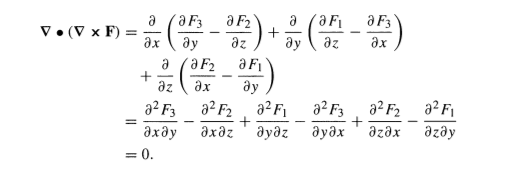
\includegraphics[scale=0.7]{image1.png}

 Tous les termes s'annulent deux à deux.
 \item
 \[\rot ( \gradt\phi) =0 = \nabla \times ( \nabla \phi ) \]

 \end{itemize}
 \subsection{Terminologie}
\begin{itemize}


\item
 $\divt F = 0$ dans $D \Leftrightarrow F$ est un champ vectoriel \og solénoïdal \fg{} ou encore \og incompressible \fg{} dans D;

\item $\rot F = 0$ dans $D \Leftrightarrow F$ est un champ vectoriel \og irrotationnel \fg{} dans $D$.

\end{itemize}
\textit{ Exemples physiques :} \\

 $\vec F= \vec B$ (le champ magnétique). $\divt B = 0$

 $\vec F= \vec V$ (la vitesse du fluide). $\divt V = 0$

 Si le fluide est incompressible $\Leftrightarrow$ Densité constante (m/vol).
 
 \textit{ Exemple} :

 \[F= \gradt \phi = \nabla \phi \textit{ (conservatif) }\]

 \[\rot F = \rot ( \gradt \phi ) =0\]

 \begin{mytheo}
 Un champ de vecteurs conservatif est irrotationnel.
 \end{mytheo}

 \[\divt ( \rot G ) = 0\]

 Si on appelle $rot G = F$.

 \begin{mytheo}
 Le rotationnel d'un champ vectoriel est solénoïdal/incompressible.
 \end{mytheo}


 \begin{mytheo}
 C'est la réciproque du théorème 1.


 Un champ de vecteurs irrotationnel est conservatif.
 \end{mytheo}


 \begin{mytheo}
C'est la réciproque du théorème 2.

 Un champ vectoriel solénoïdal ou incompressible dérive d'un potentiel vecteur : $\exists G$ tel que $\vec F = \rot \vec G$.
 \end{mytheo}
 \begin{myrem}

Pour prouver qu'un champ vectoriel est un grand $\vec f $ tel que $\vec f = \gradt F$, il faut que le domaine soit simplement connexe et que $\rot F=0$. Pour vérifier cela, il suffit d'utiliser la définition du $\rot$.

 \end{myrem}
 Ces réciproques sont vraies si le domaine D de définition du champ $\vec F$ satisfait à certaines conditions. Les réciproques ne sont pas toujours vraies, quel que soit le domaine.

 Nous allons démontrer que les réciproques sont vraies pour $D$ = ouvert, simplement connexe, \textbf{étoilé}


 \textit{Réciproque du Théorème 1} : Hypothèse : $\rot \vec F =0$

 \[\rot \vec F
=\left( \frac{\partial F_3}{\partial y } -  \frac{\partial F_2}{\partial z }\right) \xunit
+\left( \frac{\partial F_1}{\partial z } -  \frac{\partial F_3}{\partial x }\right) \yunit
+\left( \frac{\partial F_2}{\partial x } -  \frac{\partial F_1}{\partial y }\right) \zunit
\]

 On suppose que chaque composante est nulle.

 Donc,
 \[\frac{\partial F_i}{\partial x_i}=\frac{\partial F_j}{\partial x_j}\]


Cf. les conditions évoquées dans le théorème de Poincaré. Donc, si on parvient à démontrer la réciproque du théorème 1, on aura démontré le théorème de Poincaré.

D doit être ouvert simplement connexe pour que Poincaré soit vrai.\\




\textit{
Démonstration constructive :}
\textit{
Hypothèse :}

\begin{itemize}
\item $F$ irrotationnel $\Leftrightarrow \rot F =0$;
\item $D$ ouvert, simplement connexe, étoilé.
\end{itemize}

\begin{mydef}[Un domaine étoilé]

$\exists P_0 \in D : \forall P \in D $ le segment de droite $(P_0+t( P-P_0))$, avec $t\in [0,1]$ est entièrement contenu dans D. Voir image.\\

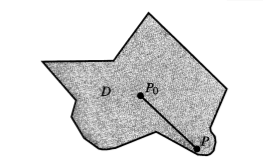
\includegraphics[scale=1]{image2.png}\\
\end{mydef}

$P_0 = (0,0,0)$ ; $\vec r(t) = (tx)\xunit + (ty) \yunit +(tz) \zunit$

$P=(x,y,z)$

On doit montrer que F est conservatif. $\exists \phi : \vec F = \nabla \phi $

\[\Leftrightarrow F_1=\frac{\partial \phi}{\partial x}\quad;\quad F_2=\frac{\partial \phi}{\partial y}\quad;\quad F_3=\frac{\partial \phi}{\partial z}\]

$\forall(x,y,z)\in D$

\[\phi(x,y,z) = \int_{P_0-P} \vec F \cdot \vec \dif r \] On a supposé que le domaine était étoilé.

\[\phi(x,y,z) = \int _{t=0} \left( F\cdot \frac{\dif r}{\dif t} \dif t \right) \]

\[\frac{\dif r}{\dif t} = (x) \xunit +(y)\yunit +(z) \zunit\]

On pose $\alpha = tx$; $\beta = ty $ ; $\gamma = tz$

Dans le livre, il y a d'autres notations.

Notons que $\frac{\partial \alpha}{\partial t} = x$

On a donc

\[\phi (x,y,z) = \int_0^1 \left( x F_1 (\alpha, \beta, \gamma ) + y F_2 + z F_3 \right) \dif t \]

On va calculer

\[\frac{\partial \phi}{\partial x} = \int_0^1 \frac{\partial}{\partial x} \left( x F_1 (\alpha, \beta, \gamma ) + y F_2 + z F_3 \right) \dif t\]

\[= \int_0^1 \left( 1F_X +X \frac{\partial F_1}{\partial x} + y \frac{\partial F_2}{\partial x} + z \frac{\partial F_3}{\partial x} \right) \dif t\]


\[
\frac{\partial F_1}{\partial x} = \frac{\partial F_1}{\partial \alpha} \frac{\partial \alpha}{\partial x}
=\frac{\partial F_1}{\partial \beta} \frac{\partial \beta}{\partial x}
=\frac{\partial F_1}{\partial \gamma} \frac{\partial \gamma}{\partial x}
\]

Or on a,

\[\frac{\partial F_1}{\partial x} = t \frac{\partial F_1}{\partial \alpha}\]

\[\frac{\partial F_2}{\partial x} = t \frac{\partial F_2}{\partial \alpha}\]

\[\frac{\partial F_3}{\partial x} = t \frac{\partial F_3}{\partial \alpha}\]

On trouve donc

\[\frac{\partial \phi}{\partial x}=\int_0^1 \left( F_1+t \frac{\partial F_1}{\partial \alpha} \frac{\partial \alpha}{\partial t}
+t \frac{\partial F_2}{\partial \alpha} \frac{\partial \\beta}{\partial t}
+t \frac{\partial F_3}{\partial \alpha} \frac{\partial \gamma}{\partial t}
\right) \dif t
\]

Cependant, par hypothèse, $\rot \vec F = 0$

\[\Leftrightarrow  \frac{\partial F_2}{\partial \alpha} = \frac{\partial F_1}{\partial \beta} \text{ et }  \frac{\partial F_3}{\partial \alpha} = \frac{\partial F_1}{\partial \gamma} \]

On trouve alors

\[
\frac{\partial \phi}{\partial x}=\int_0^1 \left( F_1 +t \frac{\partial F_1}{\partial \alpha} \frac{\partial \alpha}{\partial t}
+t \frac{\partial F_1}{\partial \beta} \frac{\partial \\beta}{\partial t}
+t \frac{\partial F_1}{\partial \gamma} \frac{\partial \gamma}{\partial t}
\right) \dif t
\]

\[=\int_0^1 \frac{\dif }{\dif t}[t F_1 ( \alpha, \beta, \gamma ) ] \dif t \]

On peut démontrer aussi pour $F_2 $ et $F_3$

\[ = tF_1 ( tx,ty,tz) \textit{entre 0 et 1} = F_1 (x,y,z) - 0\]

\begin{myrem}

Théorème 2 : Si G est un potentiel vecteur de $\vec F$, alors $(G+\nabla \phi )$ l'est aussi. $\nabla \phi$ est un champ de vecteurs conservatif.
$\rot ( G+\nabla \phi )  = \rot G + \rot ( \nabla  \phi )$ avec $\rot ( \nabla  \phi )=0$
\end{myrem}


Le potentiel vecteur est défini à un vecteur conservatif près.

\section{Les Théorèmes Intégraux}


Voici les trois raisons pour lesquelles on voit ces théorèmes :
\begin{itemize}
\item Utiles et fondamentaux pour la suite (``physique des milieux continus'');
\item Permettent de donner une interprétation intuitive à $\divt$ et $\rot$;
\item Permettent de passer d'un type d'intégrale à un autre. Par exemple, d'une intégrale de surface à une intégrale de contour.
\end{itemize}

Ce sont des cas particuliers d'un théorème unique dans le cadre de la théorie des formes différentielles extérieures.

\subsection{Théorème de Green dans le plan xy}

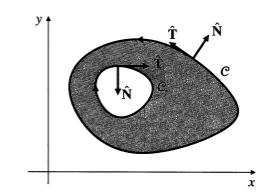
\includegraphics[scale=1]{image3.png}
\\
R est une surface orientée $ \hat N = \zunit$ et C = bord orienté.

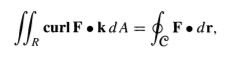
\includegraphics[scale=0.7]{image4.png}\\

\[F=F_1(x,y)\xunit +F_2(x,y)\yunit\]

On peut réécrire le Théorème de Green comme ceci\\
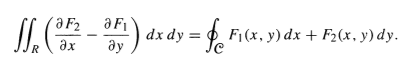
\includegraphics[scale=0.7]{image5.png}\\
\textit{
Exemple 1 : }

$\vec F=x\yunit$ (1), $\vec F = -y \xunit$(2) et $\vec F = 0.5 ( -y \xunit +x \yunit )$ (3)

Pour les trois exemples, on obtient \[\frac{\partial F_2}{\partial x}- \frac{\partial F_1}{\partial y} = 1\]

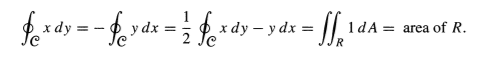
\includegraphics[scale=0.7]{image6.png}\\

Merci Green !

Appliqué à un disque elliptique :

\textit{
Exemple 2 : }\\
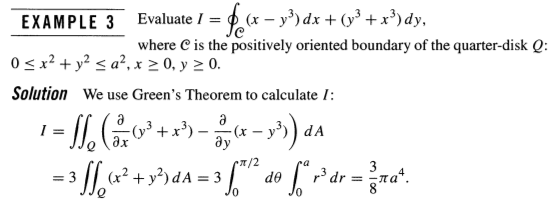
\includegraphics[scale=0.7]{image7.png}\\

\begin{myrem}

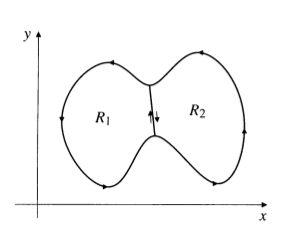
\includegraphics[scale=0.8]{image8.png}

\[\int_+ F\cdot \dif r = - \int_- F\cdot \dif r\]

Si on considère l'union des deux domaines, le théorème de Green est valable sur l'union des deux domaines. En fait, on a fait une \textbf{coupure fictive de $R$}.
\end{myrem}

\graphicspath{{CM6/}}
\part{Cours Magistral 6 -- Les intégrales}
\section{Rappel}

Théorème de Green

\begin{center}
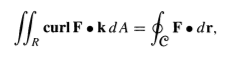
\includegraphics[scale=0.7]{image1.png}\\
\end{center}

où k = $\hat N$ et $kdA = dS$
Le théorème de Green fait le lien entre l'intégrale de surface et l'intégrale d'un contour fermé.


\section{Théorème de Stokes}

C'est une généralisation du théorème de Green

Nous avons une surface orientable par un vecteur normal.

\[\iint_S rot F\bullet \hat N dS = \oint F\bullet dr\]
\textit{Pour la démonstration, voire Adams page 914}

Ce théorème va nous donner un sens au $rot F$.

On trace un cercle de centre P et de rayon $\epsilon \to 0$ On peut appliquer le théorème.

\[\iint_{S_{\epsilon}} rot F\bullet \hat N dS = \oint_{C_{\epsilon}} F\bullet dr\]

Or on a que
\[\iint_{S_{\epsilon}} rot F\bullet \hat N dS = rot F (P) \bullet \hat N (P) \iint_{S_{\epsilon}} dS\]

Et \[\iint_{S_{\epsilon}} dS\] est l'aire du disque. C'est à dire $\pi \epsilon ^2$

\[\Rightarrow rot F(P) \bullet \hat N = \lim_{\epsilon \to 0 }\frac{1}{\pi \epsilon ^2} \oint_{C_{\epsilon}}F\bullet dr\]

Que veut dire le nom "rotationnel" ?

Prenons un champ de vecteur
\[\vec F = \vec v = x \vec j +0 \vec i +0 \vec k\]

C'est la cinématique d'un écoulement de cisaillement. Nous avons un matérau fixe ainsi qu'un matériau qui avance à côtés.
Si on place une "boule" dans ce champ vectoriel, la boule va monter et elle va également avoir un mouvement de rotation tout à fait fictif. Il a un lien avce le rotationnel. Dans ce cas-ci,\[rot \vec v = \vec k\]

Il est perpendiculaire au plan et il est constant.

Faisons donc le lien entre le rotationnel d'un champ de vecteur et la vitesse angulaire de rotation locale en un point P ( de la boule citée plus haut ).

On considère le point


$P = ( r \cos \Theta, r \sin \Theta ) \vec r $

On peut trouver

\[ v = r^{\bullet} = (-r\sin \Theta \Theta^{\bullet}, r\sin \Theta \Theta^{\bullet}\]

\[v = (-y \Omega , x \Omega) \]

\[v=(-y\Omega) i + (x\Omega) j \] est la rotation de corps rigide à vitesse angulaire $\Omega$

Faisons comme si on n'avait pas le Théorème de Stokes. Calculer la criculation de v le long de $C_{\epsilon}$

$$r^{\thicksim} = (x_0+ \epsilon \cos t ) i +( Y_0 + \epsilon \sin t )j $$

pour $\Theta \le t \le 2 \pi $

On dérive pour trouver

\[\frac{d r^{\thicksim} }{dt} + ( -\epsilon \sin t ) i + ( \epsilon \cos t ) j\]

On arrive donc à

\[\oint_{C_{\epsilon}} v \bullet dr^{\thicksim} = \oint_{C_{\epsilon}} ( v \bullet \frac{dr^{\thicksim}}{dt} ) dt \]


On calcule tout ça

\[\int_0^{2\pi} \left[ (-\Omega ( x_0 + \epsilon \sin t )) ( - \epsilon \sin t ) + (\Omega ( x_0 + \epsilon \cos t))( \epsilon \cos t ) \right] dt \]

Où

$-\Omega ( x_0 + \epsilon \sin t ) = V_x$



$- \epsilon \sin t  = \dfrac{dx}{dt}$



$(\Omega ( x_0 + \epsilon \cos t)) = V_y$




$\epsilon \cos t =\frac{dy}{dt}$




\[Circ = \int_0^{2\pi} (\Omega \epsilon ( y_0 \sin t + x_0 \cos t ) + \Omega \epsilon ^2 )\bullet dt \]

avec \[ \int_0^{2\pi} (\Omega \epsilon ( y_0 \sin t + x_0 \cos t )  = 0\]


\[Circ = \int_0^{2\pi} ( \Omega \epsilon ^2 )\bullet dt = \Omega \epsilon^3 ( 2 \pi ) = (\pi \epsilon^2 )\bullet ( 2 \Omega ) \]

\begin{myrem}
$rot v : ( 2 \Omega ) k = $ est un vecteur constant

On confirme bien stokes pour $\vec F = \vec V $


\[\iint_{S_{\epsilon}} rot v \bullet \hat N dS = \iint_{S_{\epsilon}} (2\Omega) k\bullet k dS = (2 \Omega ) \pi \epsilon ^2 = \oint_{C_{\epsilon}} v\bullet dr^{\thicksim} \]

\end{myrem}

\begin{myrem}


Dans ce exemple, la circ ne dépen pas de $(x_0,y_0)$ : car ici $ rot v = $ vecteur constant
\end{myrem}

\begin{myrem}

Il y a un sens à définir une vitesse angulaire locale au point P dans un fluide en mouvement à $\vec v$ comme étant

$$\vec \Omega (P) = 0.5 rot v (P) $$

Mécanique des milieux continus
\end{myrem}

\begin{myrem}
Dans l'exemple du début du cours, les lignes de courant sont rectilignes. En plus, elle va tourner et sa vitesse sera mesurée par le rotationnel.
\end{myrem}


Le théorème de Stokes est vraiment un outil fondamental des modèles de milieux continus ( macroscopiques ). Il permet aussi de calculer des intégrales compliquées.

On trace$C$, $S_1$, $S_2$ sont tous des bords d'une même surface.

\[\oint_C F \bullet dr = \iint_{S_1}rot F \bullet N dS = \iint_{S_2}rot F \bullet N dS\]
\textit{
Exemple : }

"Utiliser Stokes deux fois."

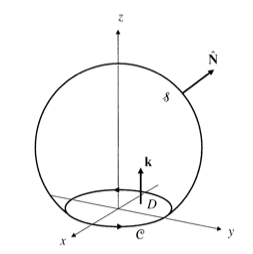
\includegraphics[scale=0.6]{image2.png}\\%Figure 16.17

C'est une sphère d'équation

\[x^2+y^2 + (z-2)^2 =8\] qui se trouve au dessus du plan ( x-y )

Le champ est le suivant
\begin{center}

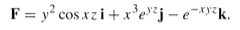
\includegraphics[scale=0.7]{image4.png}\\
\end{center}
Le vecteur normal doit être pris comme $\hat{\vec N} = \vec k $

On va prendre le disque qui forme la base de la sphère pour calculer l'intégrale. qui a pour équation $C : x^2 + y^2 = 4 $  et $S : x^2 + y^2 = 4 $ avec $S_2 \equiv 0 $


Il faut d'abord calculer le rotationnel de manière générale et puis on pose $z\equiv 0$

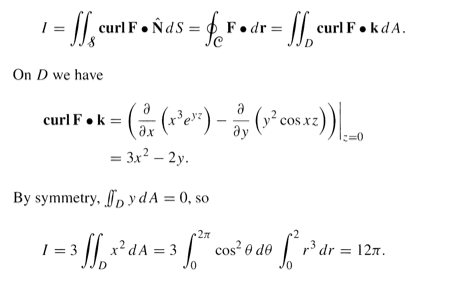
\includegraphics[scale=0.7]{image3.png}\\

\section{Théorème de la Divergence}
Ce théorème appartient à Gauss, Green, Ostrogradsky.

C'est un thèorème hyper fondamentale pour la suite.

S est une surface fermée orientée qui appartient à $\Re^3$

\[\iiint_D div F dV = \oiint_S F \bullet N dS\]
C'est une relation qui fait le lien entre une intégrale de volume de et de surface.
\textit{
Cas particulier : 2D}

\begin{center}
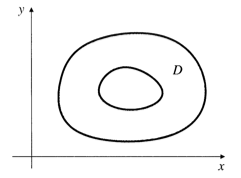
\includegraphics[scale=0.5]{image5.png}\\

\end{center}

\[\iint _R div F dA = \oint _C F \bullet N dS\]
C'est un cas particulier du thèorème de la divergence en 2D. On a pris une coupe d'un volume 3D.

\subsection{Intéprétation de div $\vec F$}

On considère une sphère de $\Re ^3$ de rayon $\epsilon \to 0$ centrée en P.

Ce qu'il va rester pour l'intégrale triple, c'est
\[div F(P) \dfrac{4\pi}{3} \epsilon^3 = \oiint _{S_{\epsilon}} F \bullet N dS \]

On voit donc que

$$div F (P) =  \lim_{\epsilon \to 0 } \frac{1}{\dfrac{4\pi}{3} \epsilon^3} \oiint _{S_{\epsilon}} F \bullet N dS $$

C'est le flux/ Volume

\subsection{Application du théorème de divergence}

\subsubsection{Calcul d'un flux}
\[\vec F = x i + y j + z k \]

Au CM4, nous avons calculer l'intégrale de flux à travers ce cylindre

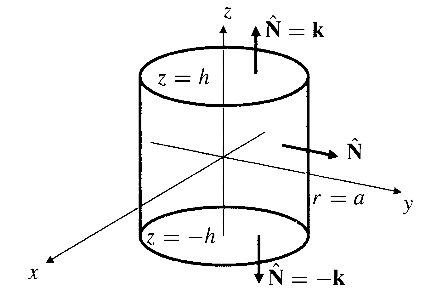
\includegraphics[scale=0.7]{image6.png}

On trouve donc

\[\iint_S F \bullet N DS = \iiint div f dV\]

On calcule donc

\[div F = \frac{\partial F_1}{\partial x}+ \frac{\partial F_2}{\partial y} + \frac{\partial F_3}{\partial z}= 1+1+1=3 = 3 \iiint dV = 6 \pi a^2 h\]

On avait obtenu la même chose au CM4

\subsubsection{Calculer $\oiint_S(x^2+y^2)dS$ sur la sphère S de rayon a centrée à l'origine}

\[x^2+y^2+z^2 = a^2\]

\begin{itemize}

\item Verifions s'il s'agit d'une intégrale de flux.

On a $\hat N = \dfrac{1}{a} r $

Or le vecteur position vaut
\[r = xi +yj +zk\]

On peut trouver
\[\dfrac{1}{a}r = \dfrac{1}{a}xi +\dfrac{1}{a}yj +\dfrac{1}{a}zk = \hat N\]

Il faut trouver F tel que $F\bullet \hat N = x^2 + y ^2 $

\[\Rightarrow F = axi +ayj +0k \]
\item Applique le théorème de la divergence

$$ I = \iiint_{Boule} div F dV = 2a \iiint_{Boule}dv$$

\[I = 2a \dfrac{4}{3}\pi a^3 = \dfrac{8}{3}\pi a^4\]
\end{itemize}

\begin{myrem}
Ne pas utiliser tel quel le Thèorème de la divergence si F n'est pas regulier dans D.


\emph{Exemple :} \[F = \dfrac{1}{||r||^3} r \] non régulier en r= 0

On établit un domaine $ D^* =D $ sans la boule centrée en 0 et puis on applique le théorème de la divergence à $D^*$

Voir Adams p910 ex 4
\end{myrem}

\begin{myrem}
\[\int_{C_{P_0 \to P_1}} \nabla f \bullet dr = f(P_1) - f(P_0) \]

\[\iint rot F \bullet dS = \oint F \bullet dr \]

\[\iiint div F dV = \oiint_S F \bullet DS\]

Ces trois théorèmes sont des généralisations des :


\[\int_a^b \frac{d}{dx}f dx = f(b) - f(a) \]

$\int$ dérivée de f = f aux bornes
\end{myrem}


\biblio


\end{document}
